\documentclass[12pt]{article}
\usepackage{graphicx}

\begin{document}
    {\Huge \textbf{Questions} \par}

    \begin{figure}[h]
        %Q15
        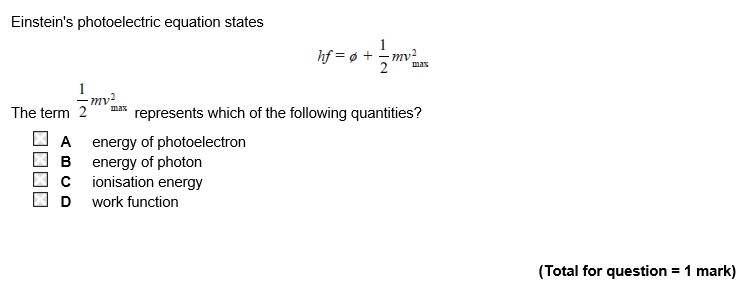
\includegraphics[width = \linewidth]{Question1.jpg}
    \end{figure}
    \begin{figure}[h]
        %Q24
        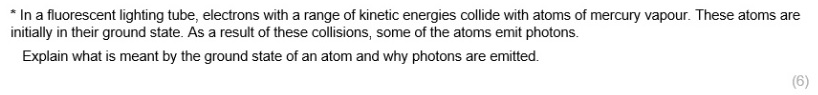
\includegraphics[width = \linewidth]{Question2.jpg}
    \end{figure}
    \begin{figure}[h]
        %Q43
        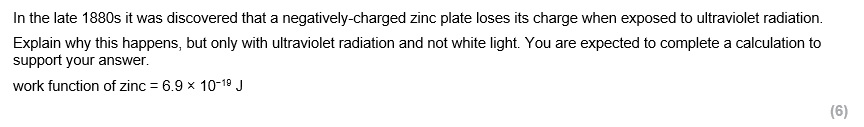
\includegraphics[width = \linewidth]{Question4.jpg}
    \end{figure}
    \begin{figure}[h]
        %Q62
        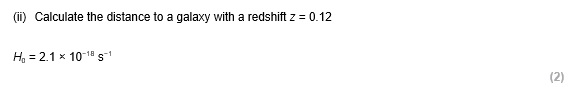
\includegraphics[width = \linewidth]{Question10.jpg}
        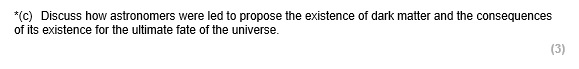
\includegraphics[width = \linewidth]{Question10P2.jpg}
    \end{figure}
    \begin{figure}[h]
        %Q37
        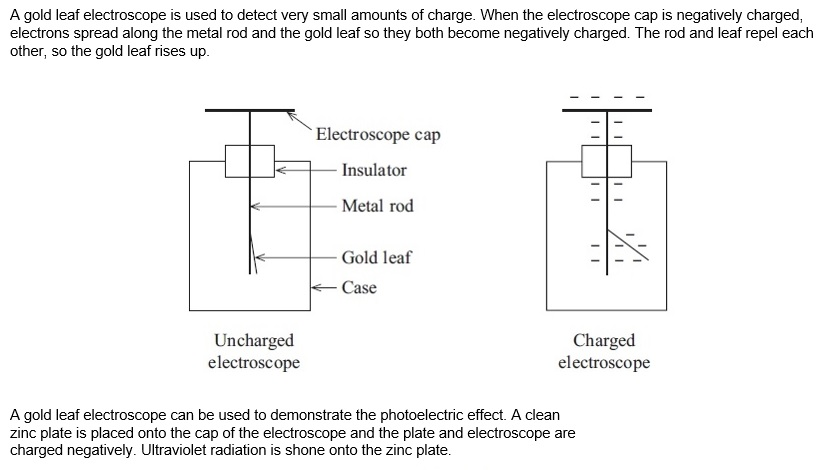
\includegraphics[width = \linewidth]{Question3P1.jpg}
        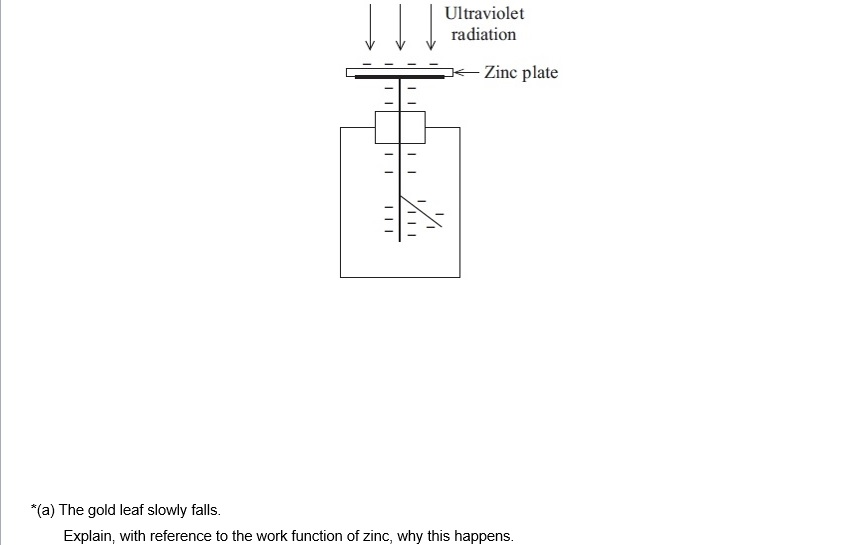
\includegraphics[width = \linewidth]{Question3P2.jpg}
        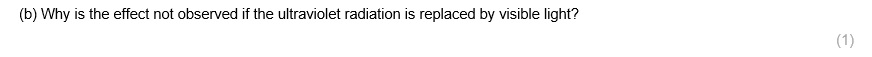
\includegraphics[width = \linewidth]{Question3P3.jpg}
        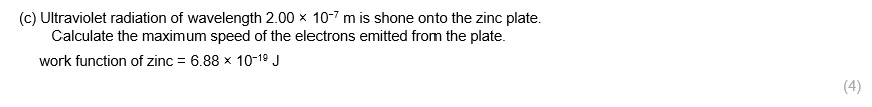
\includegraphics[width = \linewidth]{Question3P4.jpg}
        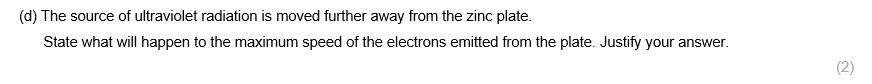
\includegraphics[width = \linewidth]{Question3P5.jpg}
    \end{figure}
    \begin{figure}[h]
        %Q41
        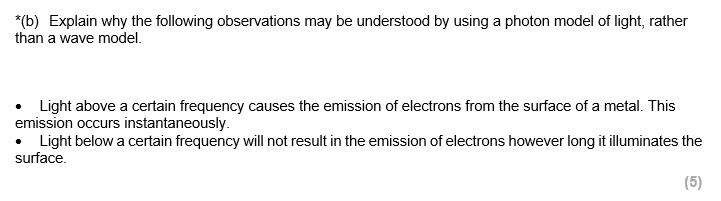
\includegraphics[width = \linewidth]{Question6.jpg}
    \end{figure}
    \begin{figure}[h]
        %Q20
        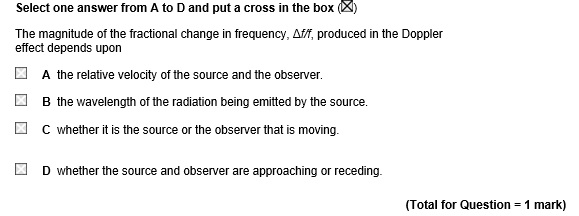
\includegraphics[width = \linewidth]{Question7.jpg}
    \end{figure}
    \begin{figure}[h]
        %Q15
        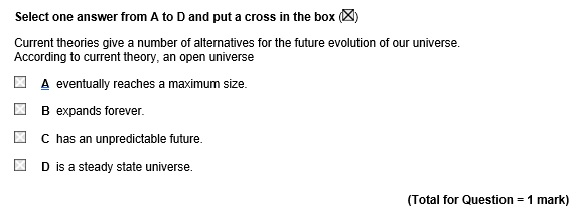
\includegraphics[width = \linewidth]{Question8.jpg}
    \end{figure}
    \begin{figure}[h]
        %Q2
        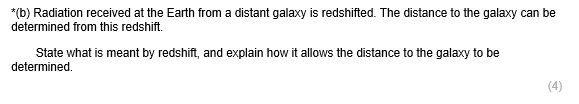
\includegraphics[width = \linewidth]{Question9.jpg}
    \end{figure}
    \end{document}